\documentclass[a4paper]{report}

\usepackage[utf8]{inputenc}
\usepackage[english]{babel}
\usepackage[T1]{fontenc}
\usepackage{textcomp}
\usepackage[]{amsthm} 
\usepackage[]{amssymb}
\usepackage{graphicx}
\usepackage{float}
\usepackage{soul}
\usepackage{color}
\usepackage{bm}
\usepackage{listings}
\usepackage{xcolor}
\usepackage{enumitem}
%\usepackage{xfrac}
\usepackage[normalem]{ulem}

% ~~~~ no indent per paragraph ~~~~-
\usepackage[parfill]{parskip}

% ~~~~ hyperlinks ~~~~ 
\usepackage[colorlinks=true, linkcolor=blue]{hyperref}

% ~~~~ subfigs ~~~~
\usepackage{subcaption}

% ~~~~ math ~~~~
\usepackage{amsmath}

\usepackage{mathtools}
% ~~ colorbox : "align" use only ~~
\newcommand{\myboxA}[1]{
	\fcolorbox{black}{lime}{#1}
}
\MakeAboxedCommand\AboxedA\myboxA

% ~~ colorbox : else ~~
\newcommand{\mybox}[1]{
	\fcolorbox{black}{lime}{$\displaystyle#1$}
}

% ~~~~ graphics ~~~~
\usepackage{tikz}
\usetikzlibrary{trees}
\usetikzlibrary {fit,shapes.geometric} % W: Command terminated with space. (1)
\usetikzlibrary {automata} % W: Command terminated with space. (1)
\usetikzlibrary{arrows.meta}
\usepackage{multicol}

\usepackage{pgfplots}
\pgfplotsset{compat = newest}

\usepackage{geometry}
\geometry{legalpaper, margin=1in}

% ~~~~ upgraded tables ~~~~
\usepackage{booktabs}

% ~~~~ algorithm formatting ~~~~
\usepackage{algorithm}
\usepackage[noend]{algpseudocode}
\usepackage{caption}

% ~~~~ list bullets ~~~~
\renewcommand{\labelitemii}{$\circ$}
\renewcommand{\labelitemiii}{$\star$}
\renewcommand{\labelitemiv}{$>$}

% figure support
\usepackage{import}
\usepackage{xifthen}
\pdfminorversion=7
\usepackage{pdfpages}
\usepackage{transparent}
\newcommand{\incfig}[1]{%
    \def\svgwidth{\columnwidth}
    \import{./figures/}{#1.pdf_tex}}

% Newline for algorithm psuedo
\newcommand{\algrule}[1][.2pt]{\par\vskip.5\baselineskip\hrule height #1\par\vskip.5\baselineskip}

% -------- Listings/XColor Settings --------
\definecolor{codegreen}{rgb}{0,0.6,0}
\definecolor{codegray}{rgb}{0.5,0.5,0.5}
\definecolor{codepurple}{rgb}{0.58,0,0.82}
\definecolor{backcolour}{rgb}{0.95,0.95,0.92}

\lstdefinestyle{mystyle}{
	backgroundcolor=\color{backcolour},
	commentstyle=\color{codegreen},
	keywordstyle=\color{magenta},
	numberstyle=\tiny\color{codegray},
	stringstyle=\color{codepurple},
	basicstyle=\ttfamily\scriptsize,
	breakatwhitespace=false,
	breaklines=true,
	captionpos=b,
	keepspaces=true,
	numbers=left,
	numbersep=5pt,
	showspaces=false,
	showstringspaces=false,
	showtabs=false,
	tabsize=4
}

\lstset{style=mystyle}

% -------------- Doc Start -------------------



\pdfsuppresswarningpagegroup=1

\title{\Huge{Hazard-Handling RISCV-I Pipeline}}
\author{\textbf{Authors:} WhisperingRock\\}
\date{CPE333\\ \small{Fall2026} \\ \today}

\begin{document}
    \maketitle

	% ~~~~ add toc as a bookmark ~~~~
	\phantomsection
	\addcontentsline{toc}{section}{\contentsname}

	\tableofcontents

	\chapter{Introduction}
		In this report, an implementation of a pipelined RISCV-I Otter 
		is constructed and improved to handle data and control hazards
		through the use of forwarding and stalling s.t. we no longer need
		to manually code \texttt{nop} in our assembly code.

	\chapter{Design}
		To properly handle data hazard Read-After-Write (RAW), we need
		to implement some way to \textit{forward} overwrite data to registers
		that need to read this data. Previously, we've used \texttt{nop} to stall
		the reading process in \textbf{EX} until the overwrite occurs in \textbf{WB}.
		Now, we can forward this data without stalling using the \textbf{Hazard Unit}
		and a few muxes.\\ Note the forwarded data is the thick orange and purple
		lines. The updated MCU can be found here \ref{otter:mcu}.

		\begin{figure}[H]
			\centering
			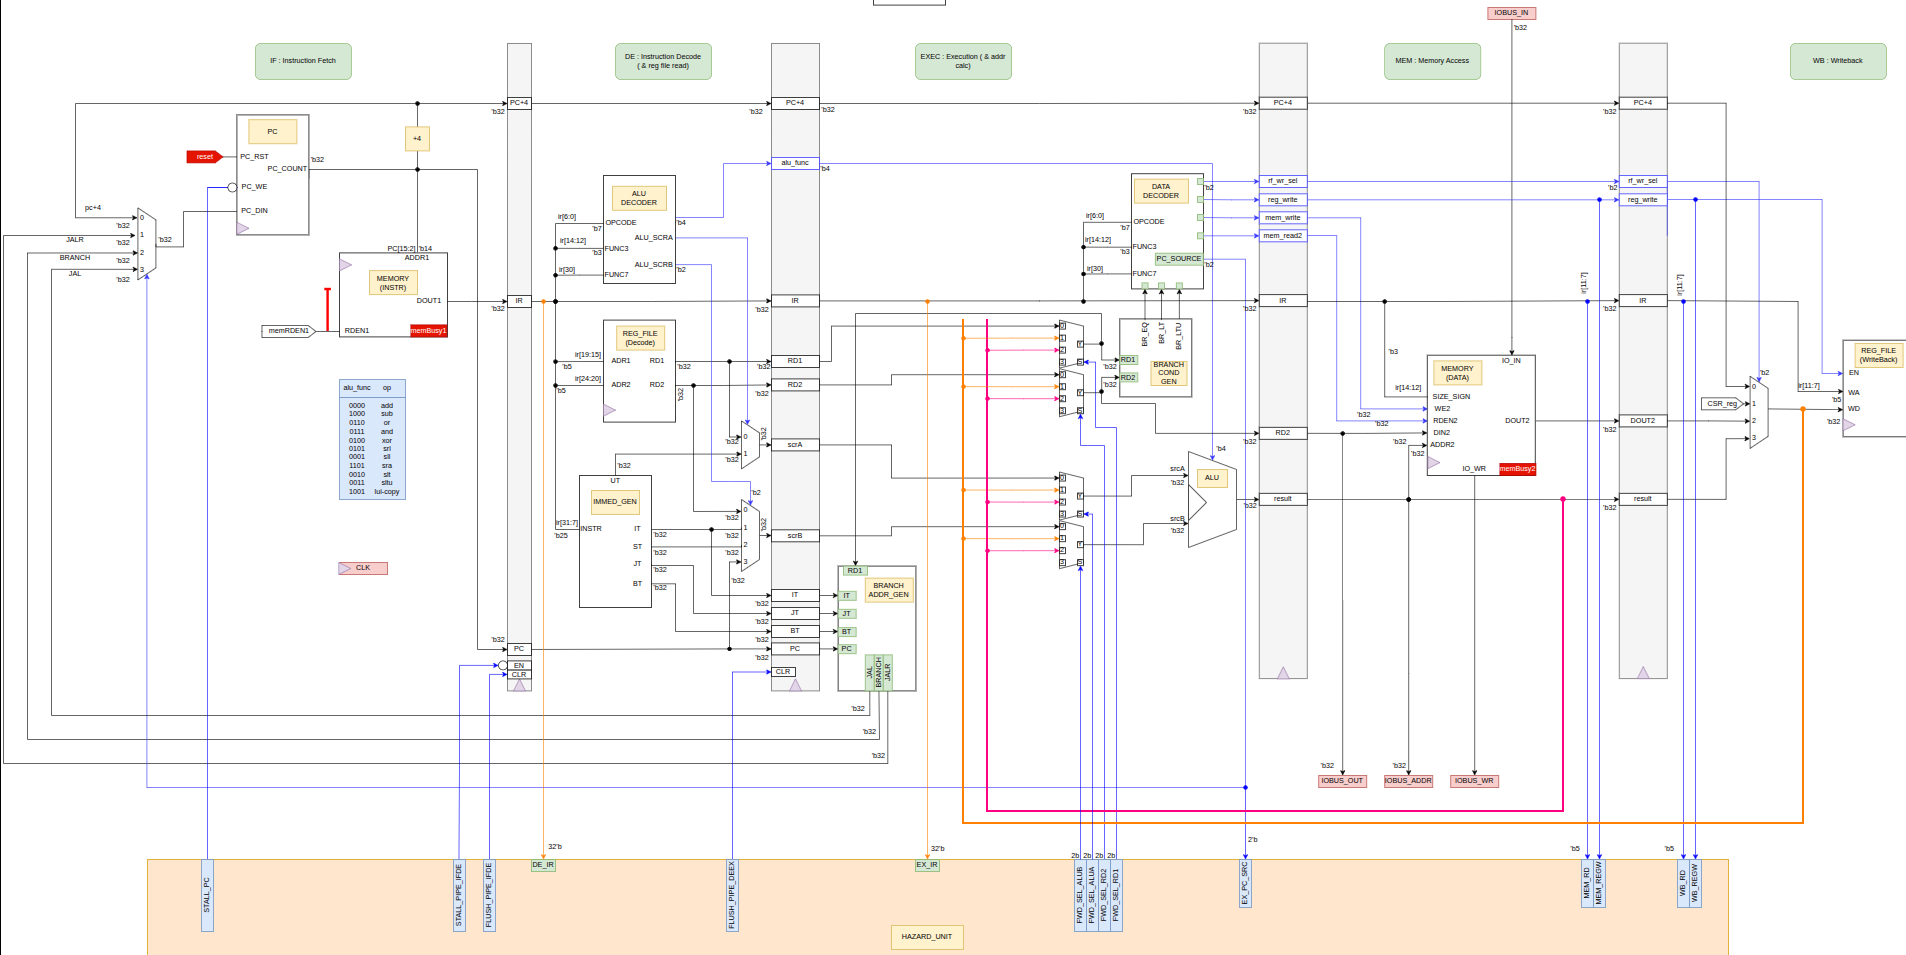
\includegraphics[
				width			=1.1 \textwidth,
				keepaspectratio	= true
			]{../../../pipeline_haz.png}
			\caption{Hazard-Handling Pipelined RISCV Otter}
			\label{fig:hazpipeotter}
		\end{figure}

		The \textbf{Hazard Unit} \ref{otter:haz} is responsible for 
		handling forwarding and stalling to prevent hazards. Figure \ref{otter:haz}
		explains how the unit flows and can be seen with the other modules
		in figure \ref{fig:hazpipeotter} as the orange block on the bottom.

		\begin{figure}[H]
			\centering
			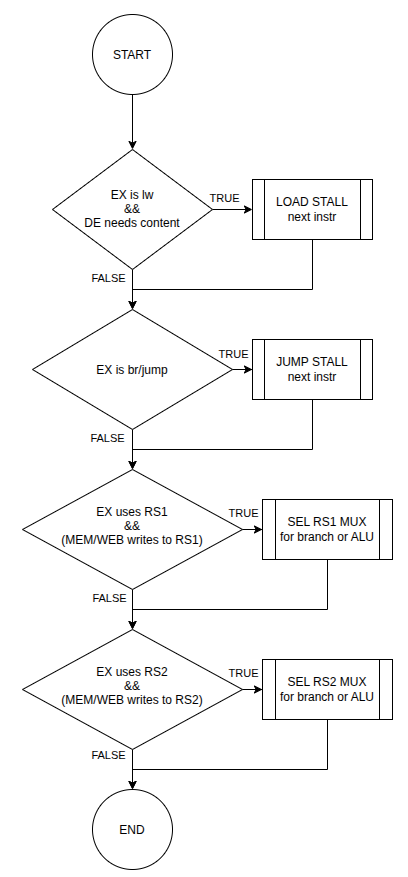
\includegraphics[
				width			= 0.35\textwidth,
				keepaspectratio	= true
			]{../../../03_labs/l4_pipeline_hazard/haz_fsm.png}
			\caption{Hazard Unit Flow Diagram}
			\label{fig:haz-flow}
		\end{figure}

		\hl{NOTE} Both memory and register file modules write on the negedge 
		rather than the posedge of the clock to meet the timing demand of
		the pipeline. See \ref{otter:rf} and \ref{otter:mem}. 

	\chapter{Testing}
		The new MCU Otter required more testing with Diego's Testall as the 
		final test. Consider :

		\begin{itemize}
			\item RAW hazards \ref{ottertest:t0}
	
				\begin{figure}[H]
					\centering
					\begin{subfigure}{\textwidth}
						\centering
						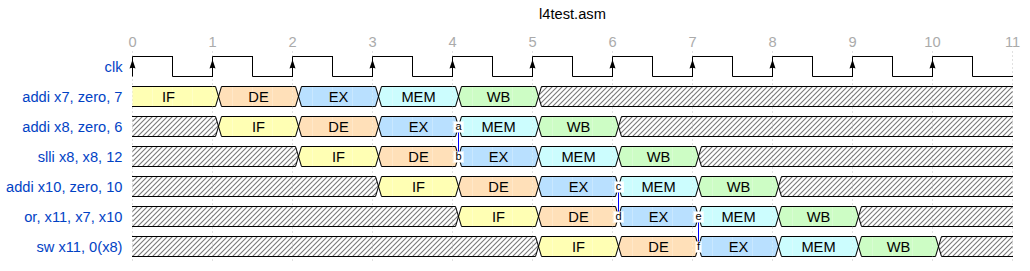
\includegraphics[
							width			= 0.8\textwidth,
							keepaspectratio	= true
						]{../exp_time_l4test.png}
						\caption{Expected Time or testfile}
						\label{fig:}
					\end{subfigure}
					\begin{subfigure}{\textwidth}
						\centering
						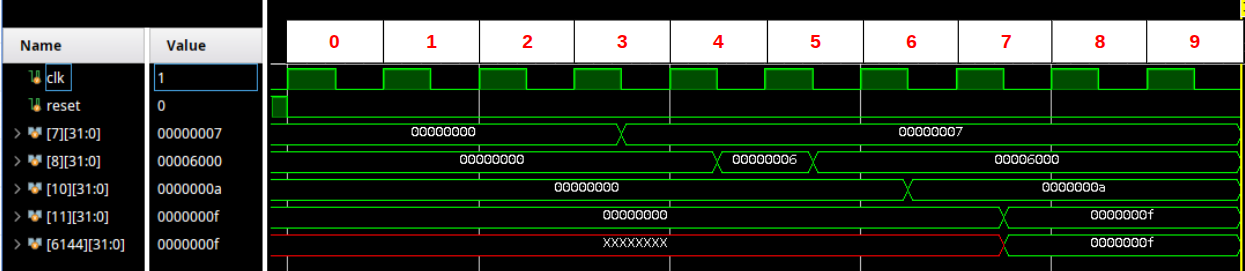
\includegraphics[
							width			= \textwidth,
							keepaspectratio	= true
						]{../act_time_l4test.png}
						\caption{Simulation Time of testfile}
						\label{fig:}
					\end{subfigure}
					\label{fig:t0}
				\end{figure}
				
				We can conclude that with our early MEM/WB writes on neg edges, 
				the expected timing matches the simulated. 

			\item RAW hazards with LOAD stalling \ref{ottertest:t1}
	
				\begin{figure}[H]
					\centering
					\begin{subfigure}{\textwidth}
						\centering
						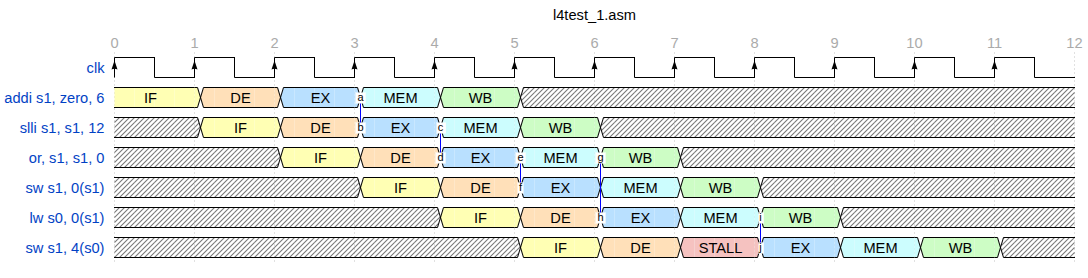
\includegraphics[
							width			= 0.9\textwidth,
							keepaspectratio	= true
						]{../exp_time_l4test1.png}
						\caption{Expected Time or testfile}
					\end{subfigure}
					\begin{subfigure}{\textwidth}
						\centering
						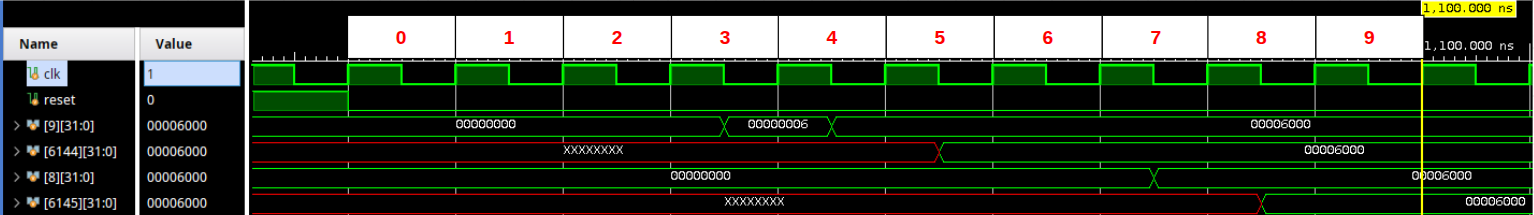
\includegraphics[
							width			= 1.1\textwidth,
							keepaspectratio	= true
						]{../act_time_l4test1.png}
						\caption{Simulation Time of testfile}
					\end{subfigure}
					\label{fig:t1}
				\end{figure}
				
				We can conclude that with our early MEM/WB writes on neg edges, 
				the expected timing matches the simulated. 

			\item RAW hazards with LOAD stalling and BRANCH flushing \ref{ottertest:t2}
	
				\begin{figure}[H]
					\centering
					\begin{subfigure}{\textwidth}
						\centering
						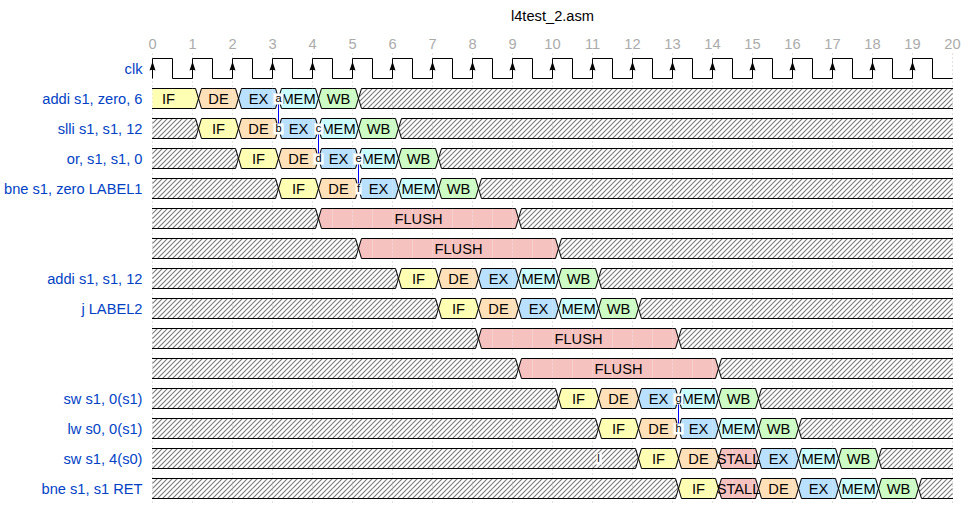
\includegraphics[
							width			= 0.9\textwidth,
							keepaspectratio	= true
						]{../exp_time_l4test2.png}
						\caption{Expected Time or testfile}
					\end{subfigure}
					\begin{subfigure}{\textwidth}
						\centering
						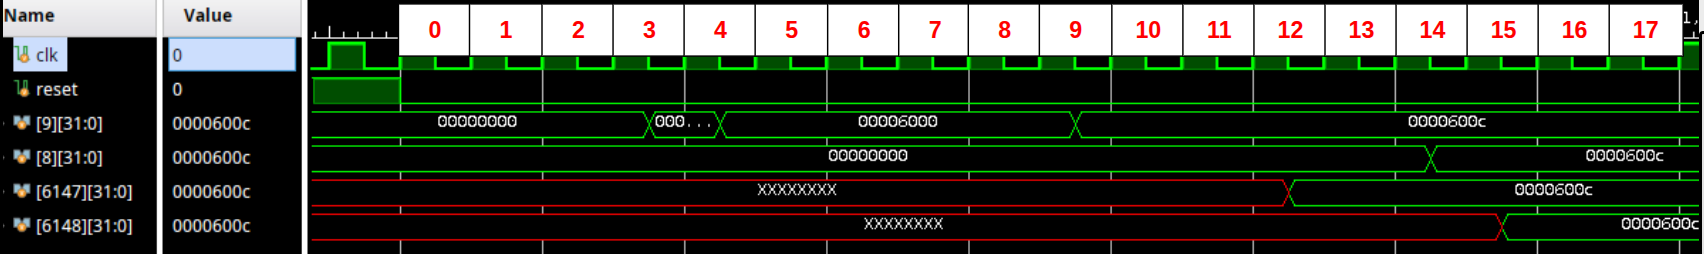
\includegraphics[
							width			= 1.1\textwidth,
							keepaspectratio	= true
						]{../act_time_l4test2.png}
						\caption{Simulation Time of testfile}
					\end{subfigure}
					\label{fig:t2}
				\end{figure}
				
				We can conclude that with our early MEM/WB writes on neg edges, 
				the expected timing matches the simulated. 

			\item Additional testing on JUMP \ref{ottertest:t3} were confirmed to pass in 
				simulation as well as Diego's Testall on hardware at 
				this point. 


		\end{itemize}
	\chapter{Results}
		After passing the basic testfiles and Diego's Testall, we must benchmark 
		the matrix multiplication program to see if we gained any latency or throughput
		boosts. Note, we should only be seeing a boost in throughput. 


	\chapter{Conclusion}
	\chapter{Appendix}
		\section{RTL Code}

			\lstinputlisting[
				language 	= {verilog},
				captionpos	= top, 
				caption		= {\texttt{HazardUnit.sv}},
				breaklines	= false, 
				label		= {otter:haz}
			]{../../../04_hardware/src/HazardUnit.sv}

			\lstinputlisting[
				language 	= {verilog},
				captionpos	= top, 
				caption		= {\texttt{Otter\_MCU\_piped.sv}},
				breaklines	= false, 
				label		= {otter:mcu}
			]{../../../04_hardware/src/Otter_MCU_piped.sv}

			\lstinputlisting[
				language 	= {verilog},
				captionpos	= top, 
				caption		= {\texttt{RegFile.sv}},
				breaklines	= false, 
				label		= {otter:rf}
			]{../../../04_hardware/src/RegFile.sv}

			\lstinputlisting[
				language 	= {verilog},
				captionpos	= top, 
				caption		= {\texttt{otter\_memory\_v1\_07.sv}},
				breaklines	= false, 
				label		= {otter:mem}
			]{../../../04_hardware/src/otter_memory_v1_07.sv}


		\section{Testing Code}
			\lstinputlisting[
				language 	= {[riscv]Assembler},
				captionpos	= top, 
				caption		= {\texttt{l4test.asm}},
				breaklines	= false, 
				label		= {ottertest:t0}
			]{../l4test.asm}

			\lstinputlisting[
				language 	= {[riscv]Assembler},
				captionpos	= top, 
				caption		= {\texttt{l4test\_1.asm}},
				breaklines	= false, 
				label		= {ottertest:t1}
			]{../l4test_1.asm}

			\lstinputlisting[
				language 	= {[riscv]Assembler},
				captionpos	= top, 
				caption		= {\texttt{l4test\_2.asm}},
				breaklines	= false, 
				label		= {ottertest:t2}
			]{../l4test_2.asm}

			\lstinputlisting[
				language 	= {[riscv]Assembler},
				captionpos	= top, 
				caption		= {\texttt{l4test\_3.asm}},
				breaklines	= false, 
				label		= {ottertest:t3}
			]{../l4test_3.asm}





\end{document}
